\section{}
\textit{Complete the numerical simulations using STAR CCM+ in the Seminar using the provided procedures. Include}
\begin{enumerate}[label=(\arabic*)]
    \item \textit{Contour of temperature}
    \item \textit{Contour of velocity}
    \item \textit{Vertical profiles of temperature and velocity}
\end{enumerate}
\textit{Furthermore, the results files of your simulations must be included in your Assignment submission.}
\subsection*{Solution}
The simulation was run as outlined in the seminar document.
\begin{figure}[h]
    \centering
    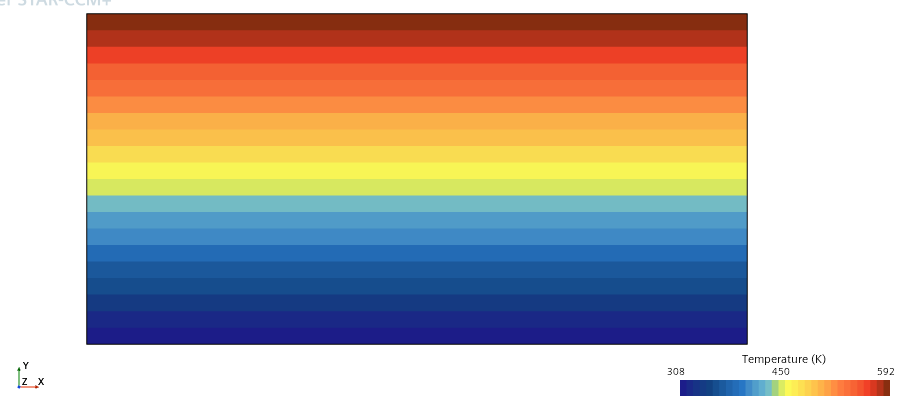
\includegraphics[width=0.8\textwidth]{Questions/Figures/Temperature Contour.png}
    \caption{Temperature Contour}
    \label{fig:Temperature Contour}
\end{figure}
\begin{figure}[h]
    \centering
    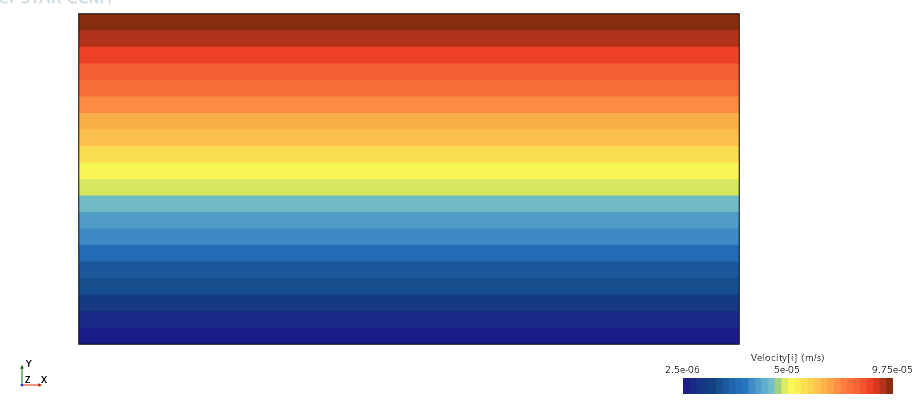
\includegraphics[width=0.8\textwidth]{Questions/Figures/Velocity Contour.png}
    \caption{Velocity Contour}
    \label{fig:Velocity Contour}
\end{figure}
\begin{figure}[h]
    \centering
    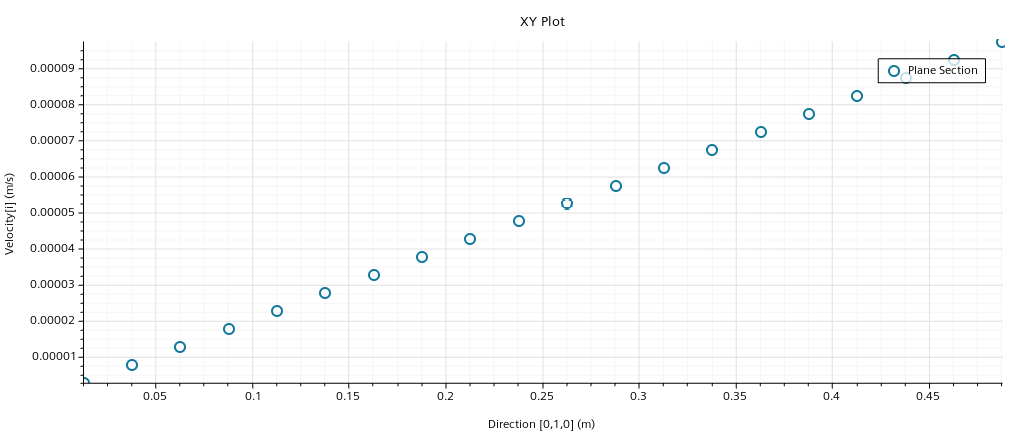
\includegraphics[width=0.8\textwidth]{Questions/Figures/Velocity Vertical Plot .png}
    \caption{Velocity Vertical Plot}
    \label{fig:Velocity Vertical Plot}
\end{figure}
\begin{figure}[h]
    \centering
    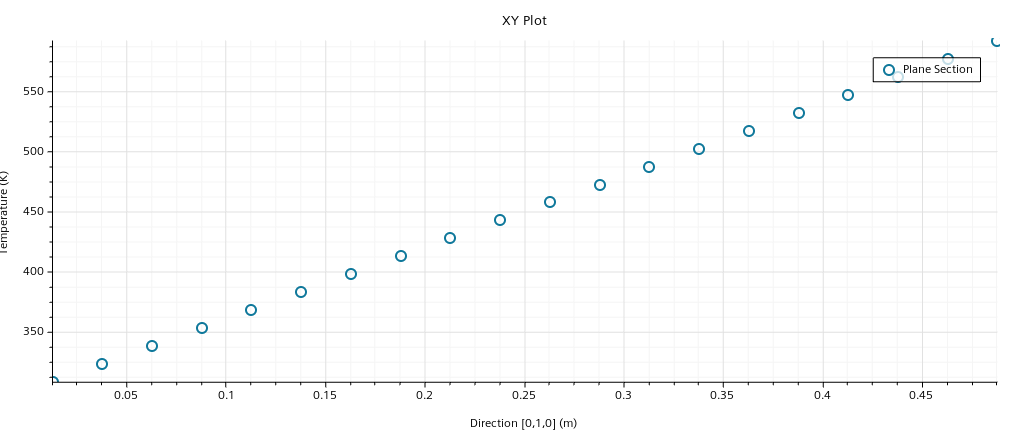
\includegraphics[width=0.8\textwidth]{Questions/Figures/Temperature Vertical Plot.png}
    \caption{Temperature Vertical Plot}
    \label{fig:Temperature Vertical Plot}
\end{figure}
\begin{figure}[h]
    \centering
    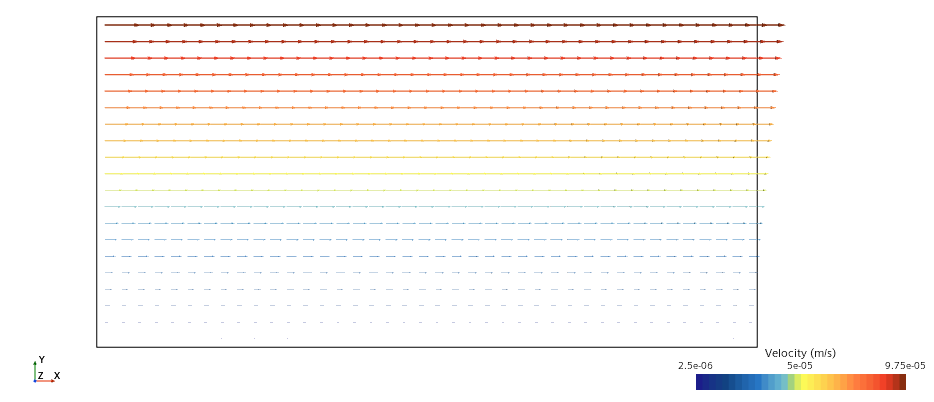
\includegraphics[width=0.8\textwidth]{Questions/Figures/Velocity Vector Profile.png}
    \caption{Velocity Vector Profile}
    \label{fig:Velocity Vector Profile}
\end{figure}
\begin{figure}[h]
    \centering
    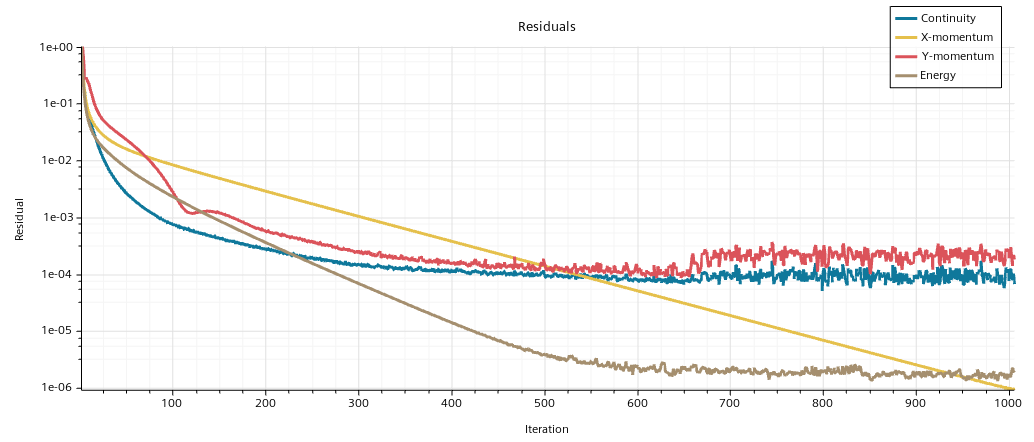
\includegraphics[width=0.8\textwidth]{Questions/Figures/Residuals.png}
    \caption{Residuals}
    \label{fig:Residuals}
\end{figure}
\FloatBarrier
\subsection*{Numerical vs Analytical Results}
The values from the problem statement were given in Table \ref{tab:Q6values}.
\begin{table}[h]
    \centering
    \caption{Parameter values}
    \begin{tabular}{cc}
        \toprule
        Variable & Value \\
        \midrule
        $u_w$ & 0.0001 m/s \\
        $H$ & 0.5 m \\
        $\mu$ & 0.001 Pa$\cdot$ s \\
        $k$ & 0.6 W/m$\cdot$ K \\
        $T_b$ & 300 K \\
        $T_u$ & 600 K \\
        \bottomrule
    \end{tabular}
    \label{tab:Q6values}
\end{table}
The analytical solution for velocity was found to be 
\begin{align*}
    u_x(y) &= \frac{u_w}{H} y \\
    &= \frac{0.0001}{0.5} y \\
    \Aboxed{&= 0.0002 y}
\end{align*}
The analytical solution for temperature was found to be
\begin{align*}
    T(y) &= a y^2 + b y + c
\end{align*}
where
\begin{align*}
    a &= -\frac{\mu}{2k} \left(\frac{u_w}{H}\right)^2 \\
    &= -\frac{0.001}{2 \cdot 0.6} \left(\frac{0.0001}{0.5}\right)^2 \\
    &= -3.33333 \times 10^{-11} \\
    b &= \frac{T_u - T_b + \frac{\mu}{2k} \left(\frac{u_w}{H}\right)^2 H^2}{H} \\
    &= \frac{600 - 300 + \frac{0.001}{2 \cdot 0.6} \left(\frac{0.0001}{0.5}\right)^2 0.5^2}{0.5} \\
    &= 600 \\
    c &= T_b \\
    &= 300
\end{align*}
so, 
\begin{align*}
    \Aboxed{T(y) &= -3.33 \times 10^{-11} y^2 + 600 y + 300}
\end{align*}
Numerical vs analytical results are compared in Tables \ref{tab:Q6velocity} and \ref{tab:Q6temperature}. Overall, the assumptions made were valid as the numerical and analytical results were in very close agreement. A linear velocity profile was observed, as expected from the Couette flow. The temperature profile had a linear profile but this is due to the small value from the viscous dissipation term. The residuals did not converge to zero, but were sufficiently small to be considered converged.

\begin{table}[h]
    \centering
    \caption{Comparison of numerical and analytical for velocity}
    \begin{tabular}{cccc}
        \toprule
        $y$ & $u_N$ & $u_A$ & Abs Difference \\
        (m) & (m/s) & (m/s) & (m/s) \\
        \midrule
        0.4875 & 9.75E-05 & 9.75E-05 & 0.00E+00 \\
        0.4625 & 9.25E-05 & 9.25E-05 & 0.00E+00 \\
        0.4375 & 8.75E-05 & 8.75E-05 & 0.00E+00 \\
        0.4125 & 8.25E-05 & 8.25E-05 & 0.00E+00 \\
        0.3875 & 7.75E-05 & 7.75E-05 & 0.00E+00 \\
        0.3625 & 7.25E-05 & 7.25E-05 & 0.00E+00 \\
        0.3375 & 6.75E-05 & 6.75E-05 & 0.00E+00 \\
        0.3125 & 6.25E-05 & 6.25E-05 & 0.00E+00 \\
        0.2875 & 5.75E-05 & 5.75E-05 & 0.00E+00 \\
        0.2625 & 5.25E-05 & 5.25E-05 & 0.00E+00 \\
        0.2375 & 4.75E-05 & 4.75E-05 & 0.00E+00 \\
        0.2125 & 4.25E-05 & 4.25E-05 & 0.00E+00 \\
        0.1875 & 3.75E-05 & 3.75E-05 & 0.00E+00 \\
        0.1625 & 3.25E-05 & 3.25E-05 & 0.00E+00 \\
        0.1375 & 2.75E-05 & 2.75E-05 & 0.00E+00 \\
        0.1125 & 2.25E-05 & 2.25E-05 & 0.00E+00 \\
        0.0875 & 1.75E-05 & 1.75E-05 & 0.00E+00 \\
        0.0625 & 1.25E-05 & 1.25E-05 & 0.00E+00 \\
        0.0375 & 7.50E-06 & 7.50E-06 & 0.00E+00 \\
        0.0125 & 2.50E-06 & 2.50E-06 & 0.00E+00 \\
        \bottomrule
    \end{tabular}
    \label{tab:Q6velocity}
\end{table}

        % y, m	vx_N, K	vx_A, K	Abs Difference
        % 0.4875	9.75E-05	9.75E-05	0.00E+00
        % 0.4625	9.25E-05	9.25E-05	0.00E+00
        % 0.4375	8.75E-05	8.75E-05	0.00E+00
        % 0.4125	8.25E-05	8.25E-05	0.00E+00
        % 0.3875	7.75E-05	7.75E-05	0.00E+00
        % 0.3625	7.25E-05	7.25E-05	0.00E+00
        % 0.3375	6.75E-05	6.75E-05	0.00E+00
        % 0.3125	6.25E-05	6.25E-05	0.00E+00
        % 0.2875	5.75E-05	5.75E-05	0.00E+00
        % 0.2625	5.25E-05	5.25E-05	0.00E+00
        % 0.2375	4.75E-05	4.75E-05	0.00E+00
        % 0.2125	4.25E-05	4.25E-05	0.00E+00
        % 0.1875	3.75E-05	3.75E-05	0.00E+00
        % 0.1625	3.25E-05	3.25E-05	0.00E+00
        % 0.1375	2.75E-05	2.75E-05	0.00E+00
        % 0.1125	2.25E-05	2.25E-05	0.00E+00
        % 0.0875	1.75E-05	1.75E-05	0.00E+00
        % 0.0625	1.25E-05	1.25E-05	0.00E+00
        % 0.0375	7.50E-06	7.50E-06	0.00E+00
        % 0.0125	2.50E-06	2.50E-06	0.00E+00
\begin{table}[h]
    \centering
    \caption{Comparison of numerical and analytical for temperature}
    \begin{tabular}{cccc}
        \toprule
        $y$ & $T_N$ & $T_A$ & Abs Difference \\
        (m) & (K) & (K) & (K) \\
        \midrule
        0.4875	& 592.5	& 592.5	& 0.00E+00 \\
        0.4625	& 577.5	& 577.5	& 6.10E-05 \\
        0.4375	& 562.5	& 562.5	& 6.10E-05 \\
        0.4125	& 547.5	& 547.5	& 0.00E+00 \\
        0.3875	& 532.5	& 532.5	& 6.10E-05 \\
        0.3625	& 517.5	& 517.5	& 6.10E-05 \\
        0.3375	& 502.5	& 502.5	& 6.10E-05 \\
        0.3125	& 487.5	& 487.5	& 6.10E-05 \\
        0.2875	& 472.5	& 472.5	& 6.10E-05 \\
        0.2625	& 457.5	& 457.5	& 3.05E-05 \\
        0.2375	& 442.5	& 442.5	& 3.05E-05 \\
        0.2125	& 427.5	& 427.5	& 3.05E-05 \\
        0.1875	& 412.5	& 412.5	& 3.05E-05 \\
        0.1625	& 397.5	& 397.5	& 3.05E-05 \\
        0.1375	& 382.5	& 382.5	& 3.05E-05 \\
        0.1125	& 367.5	& 367.5	& 0.00E+00 \\
        0.0875	& 352.5	& 352.5	& 0.00E+00 \\
        0.0625	& 337.5	& 337.5	& 0.00E+00 \\
        0.0375	& 322.5	& 322.5	& 0.00E+00 \\
        0.0125	& 307.5	& 307.5	& 0.00E+00 \\
        \bottomrule
    \end{tabular}
    \label{tab:Q6temperature}
\end{table}         

% y, m	T_N, K	T_A, K	Absolute Difference 
% 0.4875	592.5	592.5	0.00E+00
% 0.4625	577.5	577.5	6.10E-05
% 0.4375	562.5	562.5	6.10E-05
% 0.4125	547.5	547.5	0.00E+00
% 0.3875	532.5	532.5	6.10E-05
% 0.3625	517.5	517.5	6.10E-05
% 0.3375	502.5	502.5	6.10E-05
% 0.3125	487.5	487.5	6.10E-05
% 0.2875	472.5	472.5	6.10E-05
% 0.2625	457.5	457.5	3.05E-05
% 0.2375	442.5	442.5	3.05E-05
% 0.2125	427.5	427.5	3.05E-05
% 0.1875	412.5	412.5	3.05E-05
% 0.1625	397.5	397.5	3.05E-05
% 0.1375	382.5	382.5	3.05E-05
% 0.1125	367.5	367.5	0.00E+00
% 0.0875	352.5	352.5	0.00E+00
% 0.0625	337.5	337.5	0.00E+00
% 0.0375	322.5	322.5	0.00E+00
% 0.0125	307.5	307.5	0.00E+00




